\documentclass[11pt]{article}

% ---------- Packages ----------
\usepackage[a4paper,top=1in,bottom=1in,left=1in,right=1in]{geometry}
\usepackage[table]{xcolor}
\usepackage{titlesec}
\usepackage{array}
\usepackage{tabularx}
\usepackage{longtable}
\usepackage{colortbl}
\usepackage{booktabs}
\usepackage{fancyhdr}
\usepackage{enumitem}
\usepackage[T1]{fontenc}
\usepackage[utf8]{inputenc}
\usepackage{lmodern}
\usepackage{listings}
\usepackage{hyperref}
\usepackage{needspace}
\usepackage{graphicx}
\graphicspath{{IMAGES/}}

% ---------- Fonts (pdfLaTeX compatible) ----------
\renewcommand{\familydefault}{\sfdefault}

% ---------- Colors ----------
\definecolor{accent}{HTML}{5B2A86}
\definecolor{accentdark}{HTML}{3A1D5C}
\definecolor{accentlight}{HTML}{EDE7F6}
\definecolor{darkbg}{HTML}{1F2430}
\definecolor{codetext}{HTML}{E6E6E6}
\definecolor{rowalt}{HTML}{F5F0FA}
\definecolor{gray666}{HTML}{666666}
\definecolor{gray999}{HTML}{999999}
\definecolor{infosysblue}{HTML}{4A77C5}

% ---------- Section styling ----------
\titleformat{\section}
  {\normalfont\Large\bfseries\color{accent}}
  {\thesection.}{0.5em}{}
  [{\vspace{2pt}\titlerule[0.8pt]\color{black}}]
\titlespacing*{\section}{0pt}{20pt}{10pt}
\renewcommand{\thesection}{\arabic{section}}

\titleformat{\subsection}
  {\normalfont\large\bfseries\color{accentdark}}
  {\thesubsection}{0.5em}{}
\titlespacing*{\subsection}{0pt}{14pt}{6pt}

\titleformat{\subsubsection}
  {\normalfont\bfseries\itshape}
  {\thesubsubsection}{0.5em}{}
\titlespacing*{\subsubsection}{0pt}{10pt}{4pt}

% ---------- Header / Footer ----------
\pagestyle{fancy}
\fancyhf{}
\renewcommand{\headrulewidth}{0pt}
\fancyhead[R]{\small\color{gray999} BugTracker --- Module 1 Report}
\fancyfoot[C]{\small\color{gray999} Page \thepage}

% ---------- Code block environment (light theme) ----------
\lstdefinestyle{codeblock}{
  backgroundcolor=\color{accentlight},
  basicstyle=\ttfamily\footnotesize\color{accentdark},
  breaklines=true,
  columns=fullflexible,
  keepspaces=true,
  frame=leftline,
  framerule=3pt,
  rulecolor=\color{accent},
  xleftmargin=12pt,
  xrightmargin=6pt,
  framexleftmargin=8pt,
  showstringspaces=false,
  aboveskip=8pt,
  belowskip=10pt,
  literate={|}{\textbar}1
}
\lstset{style=codeblock}

% ---------- Fix: stop xcolor rowcolors bleeding into lstlisting ----------
\makeatletter
\lst@AddToHook{PreInit}{\rowcolors{0}{}{}}
\makeatother

% ---------- Table helpers ----------
\newcolumntype{L}[1]{>{\raggedright\arraybackslash}p{#1}}
\newcommand{\tblhead}[1]{\rowcolor{accent}\color{white}\bfseries #1}

% ---------- Misc ----------
\setlength{\parskip}{6pt}
\setlength{\parindent}{0pt}
\newcommand{\filelabel}[1]{\textbf{File:} \textit{\texttt{#1}}\par\vspace{2pt}}

\begin{document}

% ===================== COVER PAGE =====================
\begin{titlepage}
\thispagestyle{empty}
\begin{center}
\vspace*{3.5cm}

{\Large\bfseries\color{infosysblue} Infosys Springboard Virtual Internship 7.0}\\[2.5cm]

{\LARGE\bfseries\color{black} INTELLIGENT SOFTWARE DEFECT TRACKING}\\[0.35cm]
{\LARGE\bfseries\color{black} SYSTEM WITH RESOLUTION ASSISTANCE}\\[2.5cm]

{\large\bfseries\color{black} MODULE 1 Report:}\\[0.25cm]
{\large\bfseries\color{black} ISSUE REPORT AND FOUNDATION MANAGEMENT}\\[4cm]

{\large\color{black} Submitted By:\\[0.2cm]
Ajaykumar K R\\[0.2cm]
Batch 3 Intern}\\[2.2cm]

{\large\color{black} Submitted To:\\[0.2cm]
Dr Sumathy S\\[0.2cm]
Infosys Springboard Mentor}

\vfill
\end{center}
\end{titlepage}

\setcounter{page}{1}

% ===================== 1. EXECUTIVE SUMMARY =====================
\section{Executive Summary}

The Intelligent Software Defect Tracking System with Resolution Assistance is a full-stack web application that gives software teams a centralized platform for reporting, assigning, and resolving defects. This report documents the Module 1 deliverable, covering role-based access control, PostgreSQL-backed persistence, real-time WebSocket notifications, duplicate-issue detection, and the validated issue lifecycle.

The implementation follows a three-tier architecture: a React 19 (TypeScript) single-page application for the workspace UI, and an asynchronous FastAPI service backed by PostgreSQL for persistence, authentication, and business rules. JWT-based authentication and bcrypt password hashing secure every protected endpoint, and an auto-generated OpenAPI documentation page is served directly from the API at \texttt{/docs}.

\subsection{1.1 Scope Covered in This Report}
\begin{itemize}[leftmargin=1.5em,itemsep=2pt]
\item Role-based access control across three roles: User, Tester, Admin.
\item Issue capture with type, severity, priority, environment, and reproduction-step metadata.
\item Live client-side duplicate-issue detection using Jaccard token-overlap similarity.
\item Rule-based auto-classification of issue type and severity from the description text.
\item PostgreSQL schema for users, projects, issues, comments, attachments, notifications, and audit logs.
\item JWT authentication with bcrypt-hashed passwords and account activation/verification gates.
\item Real-time in-app notifications delivered over an authenticated WebSocket connection.
\item Comprehensive, immutable audit log with JSON field-level diffs.
\item Analytics APIs, CSV export, and admin dashboard statistics.
\item Automated backend test suite: 371 tests passing across 16 test files.
\end{itemize}

% ===================== 2. OBJECTIVE & SCOPE =====================
\section{Objective \& Scope}

Software teams commonly struggle with having no centralized place to report and track bugs, communication gaps between reporters and resolvers, no real-time visibility into status changes, difficulty assigning and monitoring work across a team, and no audit trail of who did what and when.

The objective of Module 1 is to deliver an enterprise-grade foundation that solves these problems through a structured, role-based defect-tracking platform backed by a PostgreSQL database and real-time WebSocket notifications, engineered so later milestones (AI-assisted classification, email verification, cloud deployment) require no structural rework.

\subsection{2.1 User Roles}
\renewcommand{\arraystretch}{1.3}
\rowcolors{2}{white}{rowalt}
\begin{tabular}{|L{2.6cm}|L{13.2cm}|}
\hline
\tblhead{Role} & \tblhead{What They Can Do} \\
\hline
USER & Register, log in, create bug reports, view own issues, confirm resolution, reopen issues \\
\hline
TESTER & View assigned issues, update status, resolve issues, add comments and attachments \\
\hline
ADMIN & View all issues, assign issues to testers, manage users, view analytics and audit logs \\
\hline
\end{tabular}
\endrowcolors

% ===================== 3. TECH STACK & ARCHITECTURE =====================
\section{Technology Stack \& Architecture}

The table below summarizes the stack actually used in this implementation.

\renewcommand{\arraystretch}{1.25}
\rowcolors{2}{white}{rowalt}
\begin{tabular}{|L{3.8cm}|L{9cm}|L{3cm}|}
\hline
\tblhead{Layer} & \tblhead{Technology} & \tblhead{Version} \\
\hline
Frontend & React (TypeScript) & 19.2.8 \\
\hline
Build Tool & Vite & 8.2.2 \\
\hline
Frontend Routing & React Router DOM & 7.18.2 \\
\hline
HTTP Client & Axios & 1.20.0 \\
\hline
Backend & FastAPI (Python) & 0.141.1 \\
\hline
ASGI Server & Uvicorn & 0.52.4 \\
\hline
Database ORM & SQLAlchemy (async) & 2.0.52 \\
\hline
Database & PostgreSQL & --- \\
\hline
Migrations & Alembic & 1.19.1 \\
\hline
Data Validation & Pydantic & 2.13.4 \\
\hline
Authentication & PyJWT + bcrypt & 2.13.0 / 5.0.0 \\
\hline
Real-Time & WebSockets & 17.0.1 \\
\hline
Testing & pytest + anyio & 9.1.1 / 4.14.2 \\
\hline
\end{tabular}
\endrowcolors

\subsection{3.1 Architecture Overview}

\begin{figure}[h]
  \centering
  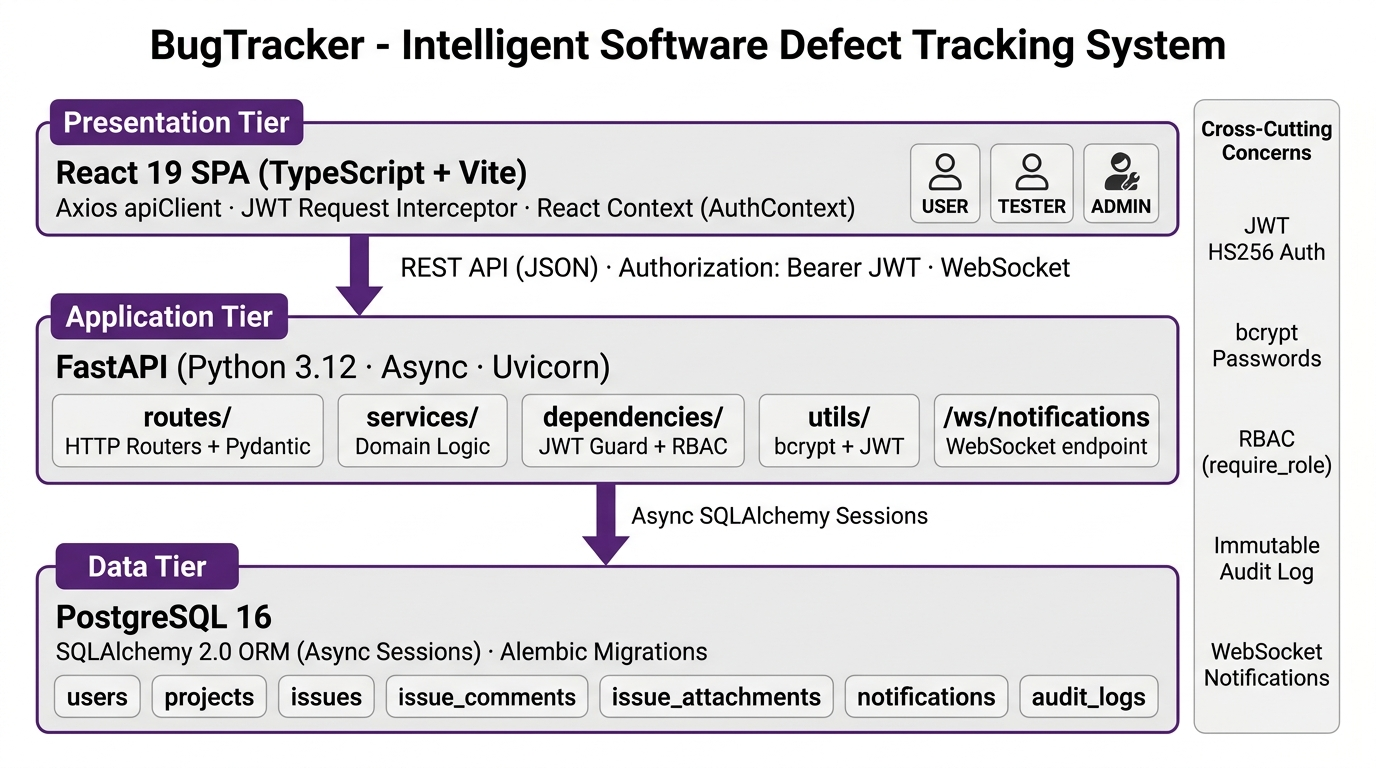
\includegraphics[width=\textwidth]{architecture.jpg}
  \caption{Three-Tier Architecture of the BugTracker System}
  \label{fig:architecture}
\end{figure}

The application follows a three-tier layered architecture:

\textbf{1. Presentation Tier} --- React 19 SPA built with TypeScript and Vite. All HTTP calls go through a centralised Axios \texttt{apiClient} with JWT injection via a request interceptor. Role-specific pages and components render based on the authenticated user role stored in React Context.

\textbf{2. Application Tier} --- FastAPI (Python 3.12, async) providing RESTful endpoints and a WebSocket endpoint. Business logic is separated into \texttt{routes/} (thin HTTP routers that validate via Pydantic schemas), \texttt{services/} (stateless domain logic --- audit logging, OTP issuance, notification dispatch), \texttt{dependencies/} (reusable JWT validation and RBAC gates), and \texttt{utils/} (JWT encode/decode, bcrypt hashing).

\textbf{3. Data Tier} --- PostgreSQL 16, accessed exclusively through SQLAlchemy 2.0 async sessions. Alembic manages schema migrations; no raw SQL strings are used --- every query is expressed through ORM constructs or Core \texttt{select()} statements.

\subsection{3.2 Project Structure}

\begin{lstlisting}
BugTracker/
|-- backend/
|   |-- app/
|   |   |-- core/            # Settings (Pydantic BaseSettings)
|   |   |-- database/        # Engine, session factory, Base class
|   |   |-- dependencies/
|   |   |   `-- auth.py      # get_current_user, require_role
|   |   |-- models/          # SQLAlchemy ORM models (one per table)
|   |   |-- routes/          # FastAPI APIRouter modules
|   |   |-- schemas/         # Pydantic request/response schemas
|   |   |-- services/        # Business logic (audit, OTP, email, notifications)
|   |   `-- utils/           # security.py (JWT + bcrypt)
|   |-- alembic/             # Migration scripts
|   `-- tests/               # 16 test files, 371 tests
|
`-- frontend/
    `-- src/
        |-- api/             # Axios instance + JWT interceptor
        |-- components/      # Reusable UI components
        |-- context/         # React context (AuthContext)
        |-- hooks/           # Custom React hooks (useAuth, etc.)
        |-- pages/           # Route-level page components
        |-- routes/          # Protected route wrappers
        |-- types/           # TypeScript interface definitions
        `-- utils/           # Formatters, PDF generator, storage helpers
\end{lstlisting}

% ===================== 4. DATABASE SCHEMA =====================
\section{PostgreSQL Database Schema}

The schema below spans seven core tables. All database interaction goes through SQLAlchemy async sessions; Alembic manages migrations.

\renewcommand{\arraystretch}{1.25}
\rowcolors{2}{white}{rowalt}
\begin{tabular}{|L{4cm}|L{11.8cm}|}
\hline
\tblhead{Table} & \tblhead{Purpose} \\
\hline
\texttt{users} & All user accounts with role, password hash, active status \\
\hline
\texttt{projects} & Software projects that issues belong to \\
\hline
\texttt{issues} & Core defect records with full classification and lifecycle fields \\
\hline
\texttt{issue\_comments} & Discussion threads on each issue \\
\hline
\texttt{issue\_attachments} & File upload metadata (binary stored on filesystem) \\
\hline
\texttt{notifications} & Persistent in-app notification records \\
\hline
\texttt{audit\_logs} & Immutable action history with JSON change diffs \\
\hline
\end{tabular}
\endrowcolors

\subsection{4.1 Core Tables}

\subsubsection{Table: users}
Stores all registered users. Passwords are stored only as bcrypt hashes; plain-text passwords are never persisted.

\begin{lstlisting}
CREATE TABLE users (
    id                SERIAL PRIMARY KEY,
    full_name         VARCHAR(200)  NOT NULL,
    email             VARCHAR(255)  NOT NULL UNIQUE,
    password_hash     VARCHAR(255)  NOT NULL,
    role              userrole      NOT NULL,
    is_active         BOOLEAN       NOT NULL DEFAULT FALSE,
    is_email_verified BOOLEAN       NOT NULL DEFAULT FALSE,
    created_at        TIMESTAMPTZ   NOT NULL DEFAULT now(),
    updated_at        TIMESTAMPTZ   NOT NULL DEFAULT now()
);
CREATE INDEX ix_users_email ON users(email);
-- userrole ENUM: ADMIN | TESTER | USER | DEVELOPER (legacy)
\end{lstlisting}

\subsubsection{Table: projects}
Groups related issues under a named project. Each issue belongs to exactly one project.

\begin{lstlisting}
CREATE TABLE projects (
    id          SERIAL PRIMARY KEY,
    project_key VARCHAR(20)   NOT NULL UNIQUE,
    name        VARCHAR(200)  NOT NULL,
    description TEXT,
    status      projectstatus NOT NULL DEFAULT 'ACTIVE',
    created_at  TIMESTAMPTZ   NOT NULL DEFAULT now(),
    updated_at  TIMESTAMPTZ   NOT NULL DEFAULT now()
);
CREATE INDEX ix_projects_project_key ON projects(project_key);
-- projectstatus ENUM: ACTIVE | INACTIVE
\end{lstlisting}

\subsubsection{Table: issues}
The central defect record, carrying the full lifecycle from REPORTED through CLOSED.

\begin{lstlisting}
CREATE TABLE issues (
    id                  SERIAL PRIMARY KEY,
    issue_key           VARCHAR(30)   NOT NULL UNIQUE,
    title               VARCHAR(500)  NOT NULL,
    description         TEXT          NOT NULL,
    issue_type          issuetype     NOT NULL DEFAULT 'BUG',
    severity            severity      NOT NULL DEFAULT 'MAJOR',
    priority            priority      NOT NULL DEFAULT 'MEDIUM',
    status              issuestatus   NOT NULL DEFAULT 'REPORTED',
    environment         VARCHAR(200),
    steps_to_reproduce  TEXT,
    expected_result     TEXT,
    actual_result       TEXT,
    resolution_summary  TEXT,
    resolved_at         TIMESTAMPTZ,
    project_id          INTEGER NOT NULL REFERENCES projects(id)  ON DELETE CASCADE,
    reporter_id         INTEGER NOT NULL REFERENCES users(id)     ON DELETE RESTRICT,
    assignee_id         INTEGER          REFERENCES users(id)     ON DELETE SET NULL,
    created_at          TIMESTAMPTZ   NOT NULL DEFAULT now(),
    updated_at          TIMESTAMPTZ   NOT NULL DEFAULT now()
);
CREATE UNIQUE INDEX ix_issues_issue_key ON issues(issue_key);
\end{lstlisting}

\renewcommand{\arraystretch}{1.25}
\rowcolors{2}{white}{rowalt}
\begin{tabular}{|L{2.6cm}|L{2.6cm}|L{10.6cm}|}
\hline
\tblhead{Column} & \tblhead{Enum Name} & \tblhead{Values} \\
\hline
issue\_type & issuetype & BUG, FEATURE\_REQUEST, ENHANCEMENT, TECHNICAL\_DEBT, SUPPORT\_TICKET \\
\hline
severity & severity & MINOR, MAJOR, CRITICAL, BLOCKER \\
\hline
priority & priority & LOW, MEDIUM, HIGH, URGENT \\
\hline
status & issuestatus & REPORTED, TRIAGED, ASSIGNED, IN\_DEVELOPMENT, IN\_REVIEW, IN\_TESTING, RESOLVED, CLOSED, REOPENED \\
\hline
\end{tabular}
\endrowcolors

\vspace{4pt}
Foreign key semantics: \texttt{project\_id} cascades (deleting a project removes its issues); \texttt{reporter\_id} restricts (a user cannot be deleted while they have reported issues); \texttt{assignee\_id} sets null on delete (leaving the issue unassigned).

\subsection{4.2 Comments \& Attachments}

\subsubsection{Table: issue\_comments}
\begin{lstlisting}
CREATE TABLE issue_comments (
    id         SERIAL PRIMARY KEY,
    issue_id   INTEGER NOT NULL REFERENCES issues(id) ON DELETE CASCADE,
    author_id  INTEGER NOT NULL REFERENCES users(id)  ON DELETE RESTRICT,
    body       TEXT    NOT NULL,
    created_at TIMESTAMPTZ NOT NULL DEFAULT now(),
    updated_at TIMESTAMPTZ NOT NULL DEFAULT now()
);
CREATE INDEX ix_issue_comments_issue_id   ON issue_comments(issue_id);
CREATE INDEX ix_issue_comments_author_id  ON issue_comments(author_id);
\end{lstlisting}

Security constraint (enforced in the service layer): \texttt{author\_id} is never accepted from the request body --- it is always set from the validated JWT token, preventing comment forgery.

\subsubsection{Table: issue\_attachments}
Stores metadata for uploaded files. Binary content lives on the filesystem; only references are stored in the database.

\begin{lstlisting}
CREATE TABLE issue_attachments (
    id                SERIAL PRIMARY KEY,
    issue_id          INTEGER       NOT NULL REFERENCES issues(id) ON DELETE CASCADE,
    uploaded_by       INTEGER       NOT NULL REFERENCES users(id)  ON DELETE RESTRICT,
    original_filename VARCHAR(500)  NOT NULL,
    stored_filename   VARCHAR(500)  NOT NULL UNIQUE,
    storage_path      VARCHAR(1000) NOT NULL,
    mime_type         VARCHAR(200)  NOT NULL,
    file_size         BIGINT        NOT NULL,
    created_at        TIMESTAMPTZ   NOT NULL DEFAULT now()
);
\end{lstlisting}

\subsection{4.3 Notifications \& Audit Log}

\subsubsection{Table: notifications}
\begin{lstlisting}
CREATE TABLE notifications (
    id                SERIAL PRIMARY KEY,
    user_id           INTEGER          NOT NULL REFERENCES users(id) ON DELETE CASCADE,
    notification_type notificationtype NOT NULL,
    title             VARCHAR(200)     NOT NULL,
    message           TEXT             NOT NULL,
    entity_type       VARCHAR(50),
    entity_id         INTEGER,
    entity_key        VARCHAR(100),
    is_read           BOOLEAN          NOT NULL DEFAULT FALSE,
    read_at           TIMESTAMPTZ,
    created_at        TIMESTAMPTZ      NOT NULL DEFAULT now()
);
CREATE INDEX ix_notifications_user_id_is_read ON notifications(user_id, is_read);
\end{lstlisting}

\texttt{notificationtype} enum values: ISSUE\_ASSIGNED, ISSUE\_STATUS\_CHANGED, ISSUE\_RESOLVED, ISSUE\_REOPENED, ISSUE\_COMMENTED, ISSUE\_MENTIONED, ATTACHMENT\_ADDED, USER\_ROLE\_CHANGED, USER\_ACTIVATED, USER\_DEACTIVATED.

\subsubsection{Table: audit\_logs}
An immutable, chronological record of every significant action in the system. No UPDATE or DELETE API is exposed for this table.

\begin{lstlisting}
CREATE TABLE audit_logs (
    id          SERIAL PRIMARY KEY,
    user_id     INTEGER      REFERENCES users(id) ON DELETE SET NULL,
    action      auditaction  NOT NULL,
    entity_type VARCHAR(50)  NOT NULL,
    entity_id   INTEGER,
    entity_key  VARCHAR(100),
    description TEXT         NOT NULL DEFAULT '',
    old_values  JSONB,
    new_values  JSONB,
    created_at  TIMESTAMPTZ  NOT NULL DEFAULT now()
);
CREATE INDEX ix_audit_logs_entity_type_action ON audit_logs(entity_type, action);
CREATE INDEX ix_audit_logs_created_at_desc    ON audit_logs(created_at DESC);
\end{lstlisting}

\renewcommand{\arraystretch}{1.25}
\rowcolors{2}{white}{rowalt}
\begin{tabular}{|L{3.2cm}|L{12.6cm}|}
\hline
\tblhead{Category} & \tblhead{Actions} \\
\hline
Authentication & AUTH\_LOGIN, AUTH\_LOGOUT \\
\hline
User management & USER\_UPDATED, USER\_ACTIVATED, USER\_DEACTIVATED, USER\_ROLE\_CHANGED \\
\hline
Comments & COMMENT\_CREATED, COMMENT\_UPDATED, COMMENT\_DELETED \\
\hline
Attachments & ATTACHMENT\_UPLOADED, ATTACHMENT\_DELETED \\
\hline
\end{tabular}
\endrowcolors

% ===================== 5. AUTH & RBAC =====================
\section{Authentication \& Role-Based Access Control}

The system uses stateless JSON Web Tokens (JWT) signed with HS256. Tokens are issued at login and verified on every protected request without any server-side session store.

\subsection{5.1 Token Issuance}
\filelabel{backend/app/utils/security.py}

\begin{lstlisting}
def create_access_token(user_id: int, role: str) -> str:
    """Create a signed JWT access token.

    Payload:
      sub   -- str(user_id)
      role  -- user role string (e.g. "TESTER")
      iat   -- issued-at (UTC)
      exp   -- expiry (UTC, ACCESS_TOKEN_EXPIRE_MINUTES from now)
    """
    now = datetime.now(UTC)
    expire = now + timedelta(minutes=settings.ACCESS_TOKEN_EXPIRE_MINUTES)
    payload: dict[str, Any] = {
        "sub": str(user_id),
        "role": role,
        "iat": now,
        "exp": expire,
    }
    return jwt.encode(
        payload,
        settings.JWT_SECRET_KEY,
        algorithm=settings.JWT_ALGORITHM,   # HS256
    )
\end{lstlisting}

\renewcommand{\arraystretch}{1.25}
\rowcolors{2}{white}{rowalt}
\begin{tabular}{|L{2cm}|L{2.4cm}|L{11.4cm}|}
\hline
\tblhead{Claim} & \tblhead{Type} & \tblhead{Description} \\
\hline
sub & str(int) & Primary key of the authenticated user \\
\hline
role & str & User role at time of issuance (ADMIN, TESTER, USER) \\
\hline
iat & int epoch & Issued-at timestamp \\
\hline
exp & int epoch & Expiry timestamp (configurable; default 1 day) \\
\hline
\end{tabular}
\endrowcolors

\vspace{4pt}
The JWT value itself is never stored in the database. Logout is client-side (discard the token); token revocation is not implemented in this phase, consistent with the stateless design.

\subsection{5.2 Guard Middleware: get\_current\_user}
\filelabel{backend/app/dependencies/auth.py}

\begin{lstlisting}
async def get_current_user(
    credentials: Annotated[
        HTTPAuthorizationCredentials | None,
        Depends(_bearer_scheme),
    ],
    db: AsyncSession = Depends(get_db),
) -> User:
    """Return the authenticated active User, or raise 401 / 403."""
    if credentials is None:
        raise _401

    payload = decode_access_token(credentials.credentials)
    user_id_str = payload.get("sub")
    if not user_id_str or not user_id_str.isdigit():
        raise _401

    result = await db.execute(select(User).where(User.id == int(user_id_str)))
    user = result.scalar_one_or_none()
    if user is None:
        raise _401
    if not user.is_active:
        raise HTTPException(status_code=403, detail="Account is inactive.")
    return user
\end{lstlisting}

A database lookup runs on every request because the \texttt{is\_active} flag can be toggled by an admin at any time; a pure JWT check would miss this, so the DB lookup ensures deactivated accounts are rejected immediately even if their token has not expired.

\subsection{5.3 Login Endpoint}
\filelabel{backend/app/routes/auth.py}

Login security measures: (1) user-enumeration prevention --- the same ``Invalid email or password.'' message is returned whether the email does not exist or the password is wrong; (2) constant-time password comparison via bcrypt; (3) pre-issuance checks for email verification and account activation before the JWT is issued; (4) every successful login is recorded in \texttt{audit\_logs} with actor, timestamp, and description, while the JWT value itself is never logged or stored.

\subsection{5.4 Role Permission Matrix}

Permissions are enforced at two layers: the client (UI) conditionally renders buttons and navigation based on the user's role for usability, while the server independently enforces every mutation through a \texttt{require\_role(...)} dependency --- the server never trusts a client-claimed role.

\filelabel{backend/app/dependencies/auth.py}
\begin{lstlisting}
def require_role(*roles: UserRole):
    """Return a FastAPI dependency that restricts access to *roles*."""
    async def _check_role(
        current_user: User = Depends(get_current_user),
    ) -> User:
        if current_user.role not in roles:
            raise HTTPException(
                status_code=403,
                detail="You do not have permission to perform this action.",
            )
        return current_user
    return _check_role
\end{lstlisting}

\renewcommand{\arraystretch}{1.2}
\rowcolors{2}{white}{rowalt}
\begin{longtable}{|L{6.6cm}|c|c|c|}
\hline
\tblhead{Action} & \tblhead{USER} & \tblhead{TESTER} & \tblhead{ADMIN} \\
\hline
\endfirsthead
\hline
\tblhead{Action} & \tblhead{USER} & \tblhead{TESTER} & \tblhead{ADMIN} \\
\hline
\endhead
Register / Login & Yes & Yes & Yes \\ \hline
View own profile & Yes & Yes & Yes \\ \hline
Create issue & Yes & No & Yes \\ \hline
View own issues & Yes & No & Yes \\ \hline
View all issues & No & No & Yes \\ \hline
View assigned issues & No & Yes & Yes \\ \hline
Assign issue to tester & No & No & Yes \\ \hline
Update issue status & No & Yes & Yes \\ \hline
Resolve issue & No & Yes & Yes \\ \hline
Confirm / close resolved issue & Yes & No & Yes \\ \hline
Reopen issue & Yes & Yes & Yes \\ \hline
Add comment & Yes & Yes & Yes \\ \hline
Edit / delete own comment & Yes & Yes & Yes \\ \hline
Delete any comment & No & No & Yes \\ \hline
Upload attachment & Yes & Yes & Yes \\ \hline
Delete attachment & No & Yes & Yes \\ \hline
Manage users (activate/deactivate/role) & No & No & Yes \\ \hline
View audit logs & No & No & Yes \\ \hline
View analytics & No & No & Yes \\ \hline
\end{longtable}
\endrowcolors

{\small\itshape\color{gray666} ``No'' denotes an action blocked at the server layer with HTTP 403.}

% ===================== 6. DUPLICATE DETECTION =====================
\section{Duplicate Detection \& Auto-Classification}

\subsection{6.1 Similarity Scoring}
\filelabel{frontend/src/pages/IssuesPage.tsx}

As a user types a new issue title in the Report Issue modal, the frontend performs client-side, real-time similarity scoring against every issue already loaded in the current session --- giving instant feedback with no extra API round-trip. The scoring uses Jaccard similarity over tokenised word sets: $\text{similarity}(A, B) = |tokens(A) \cap tokens(B)| / |tokens(A) \cup tokens(B)|$. Titles normalise to lowercase with punctuation stripped, and scores of 0.4 or higher surface as potential duplicates.

\begin{lstlisting}
function tokenize(text: string): Set<string> {
  return new Set(
    text.toLowerCase().replace(/[^a-z0-9\s]/g, '').split(/\s+/).filter(Boolean)
  );
}

function jaccardSimilarity(a: string, b: string): number {
  const setA = tokenize(a);
  const setB = tokenize(b);
  if (setA.size === 0 && setB.size === 0) return 1;
  const intersection = new Set([...setA].filter(x => setB.has(x)));
  const union = new Set([...setA, ...setB]);
  return intersection.size / union.size;
}

const DUPLICATE_THRESHOLD = 0.4;
const similarIssues = issues
  .filter(issue => jaccardSimilarity(formTitle, issue.title) >= DUPLICATE_THRESHOLD)
  .sort((a, b) => jaccardSimilarity(formTitle, b.title) - jaccardSimilarity(formTitle, a.title))
  .slice(0, 3);
\end{lstlisting}

When \texttt{similarIssues.length > 0}, a warning panel renders below the title field with clickable links to the matching issues. The user can dismiss the warning and submit anyway --- the check is advisory, not a hard block.

\subsection{6.2 Auto-Classification}

Once the description reaches 10 characters, a lightweight rule-based classifier auto-suggests the Issue Type and Severity fields. The dropdowns auto-update to the suggested values, with an info banner explaining the suggestion; the user can change either field.

\begin{lstlisting}
const SEVERITY_KEYWORDS: Record<Severity, string[]> = {
  BLOCKER:  ['crash', 'down', 'data loss', 'cannot login', 'unrecoverable'],
  CRITICAL: ['error', 'fail', 'broken', 'not working', 'exception', '500'],
  MAJOR:    ['wrong', 'incorrect', 'missing', 'unexpected', 'slow'],
  MINOR:    ['typo', 'cosmetic', 'alignment', 'colour', 'color', 'spacing'],
};

const TYPE_KEYWORDS: Record<IssueType, string[]> = {
  BUG:             ['bug', 'error', 'fail', 'crash', 'broken', 'wrong'],
  FEATURE_REQUEST: ['feature', 'request', 'add', 'new', 'want', 'need'],
  ENHANCEMENT:     ['improve', 'enhance', 'better', 'optimise', 'optimize'],
  TECHNICAL_DEBT:  ['refactor', 'cleanup', 'debt', 'legacy', 'migrate'],
  SUPPORT_TICKET:  ['how to', 'help', 'question', 'clarify', 'understand'],
};
\end{lstlisting}

\renewcommand{\arraystretch}{1.25}
\rowcolors{2}{white}{rowalt}
\begin{tabular}{|L{12.8cm}|L{3cm}|}
\hline
\tblhead{Trigger Words} & \tblhead{Suggested Severity} \\
\hline
crash, down, data loss, cannot login, unrecoverable & BLOCKER \\
\hline
error, fail, broken, not working, exception, 500 & CRITICAL \\
\hline
wrong, incorrect, missing, unexpected, slow & MAJOR \\
\hline
typo, cosmetic, alignment, colour, spacing & MINOR \\
\hline
\end{tabular}
\endrowcolors

\subsection{6.3 Issue Lifecycle}

\begin{figure}[htbp]
  \centering
  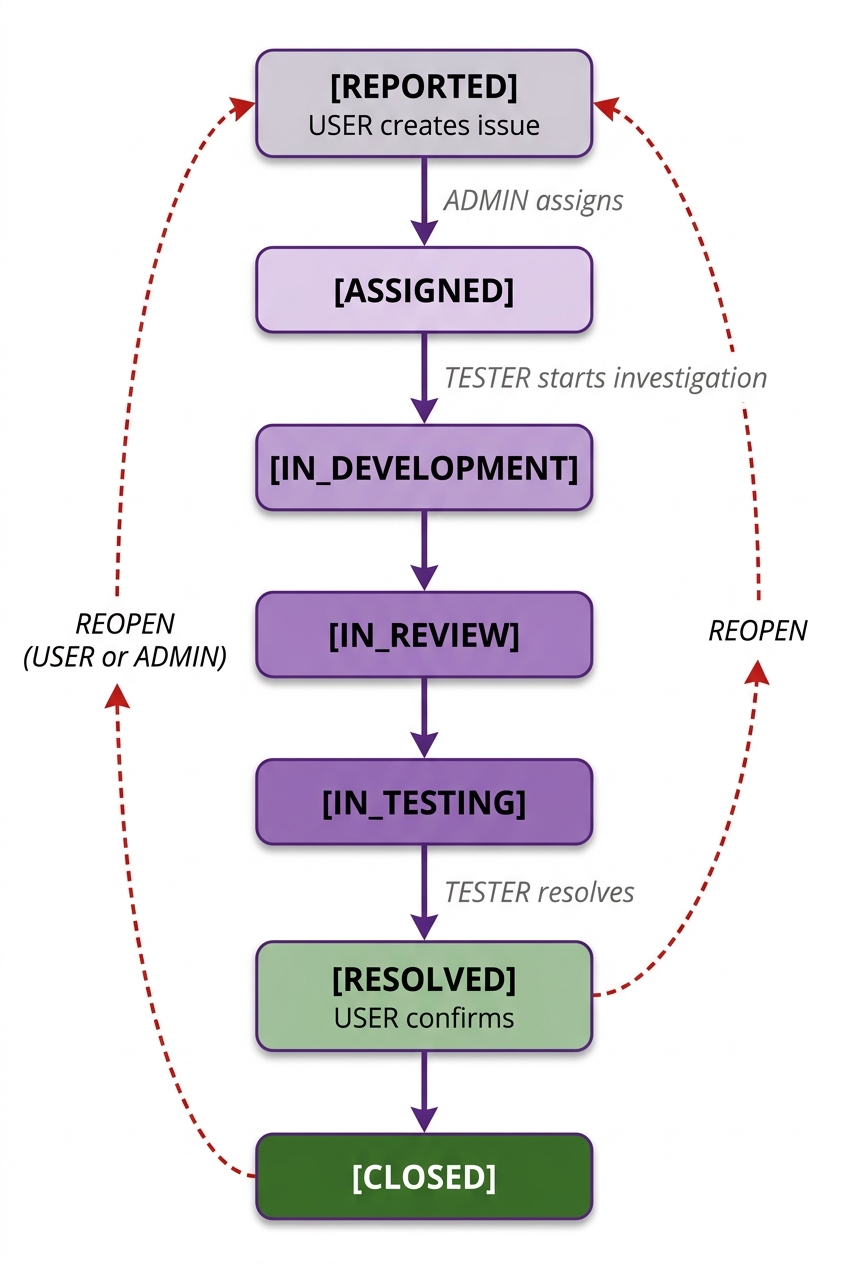
\includegraphics[width=0.52\textwidth]{lifecycle.jpg}
  \caption{Issue Lifecycle --- Status transitions from creation to closure with reopen paths}
  \label{fig:lifecycle}
\end{figure}

\texttt{resolved\_at} is stamped server-side the first time an issue enters RESOLVED, and every status change, assignment, comment, and attachment is captured in the audit log for a full trail.

% ===================== 7. REAL-TIME NOTIFICATIONS =====================
\section{Real-Time Notifications}

When an Admin assigns an issue to a Tester: a Notification record is saved to PostgreSQL; the backend pushes a JSON event to the Tester's open WebSocket connection; the Tester sees a toast popup immediately with no page refresh; and the Tester dashboard automatically refreshes to show the newly assigned issue.

The WebSocket connection (\texttt{/ws/notifications?token=<JWT>}) is secured by JWT --- the backend validates the token and derives the user ID entirely from it, never from client input.

% ===================== 8. TESTING RESULTS =====================
\section{Testing Results}

The backend test suite covers authentication, RBAC, issue lifecycle, comments, attachments, notifications, analytics, audit logs, and WebSocket connections across 16 test files.

\begin{lstlisting}
$ pytest tests/ --ignore=tests/test_e2e_workflow.py

371 passed, 11 skipped in 21.93s
\end{lstlisting}

Zero test failures. The complete end-to-end workflow (User $\rightarrow$ Admin $\rightarrow$ Tester $\rightarrow$ User) has additionally been manually verified through the browser application.

% ===================== 8b. APPLICATION SCREENSHOTS =====================
\subsection*{Application Screenshots}

The following screenshots demonstrate the live application across all three user roles.

% --- Page 1: Landing + Registration side by side ---
\clearpage
\begin{figure}[htbp]
  \centering
  \begin{minipage}[t]{0.58\textwidth}
    \centering
    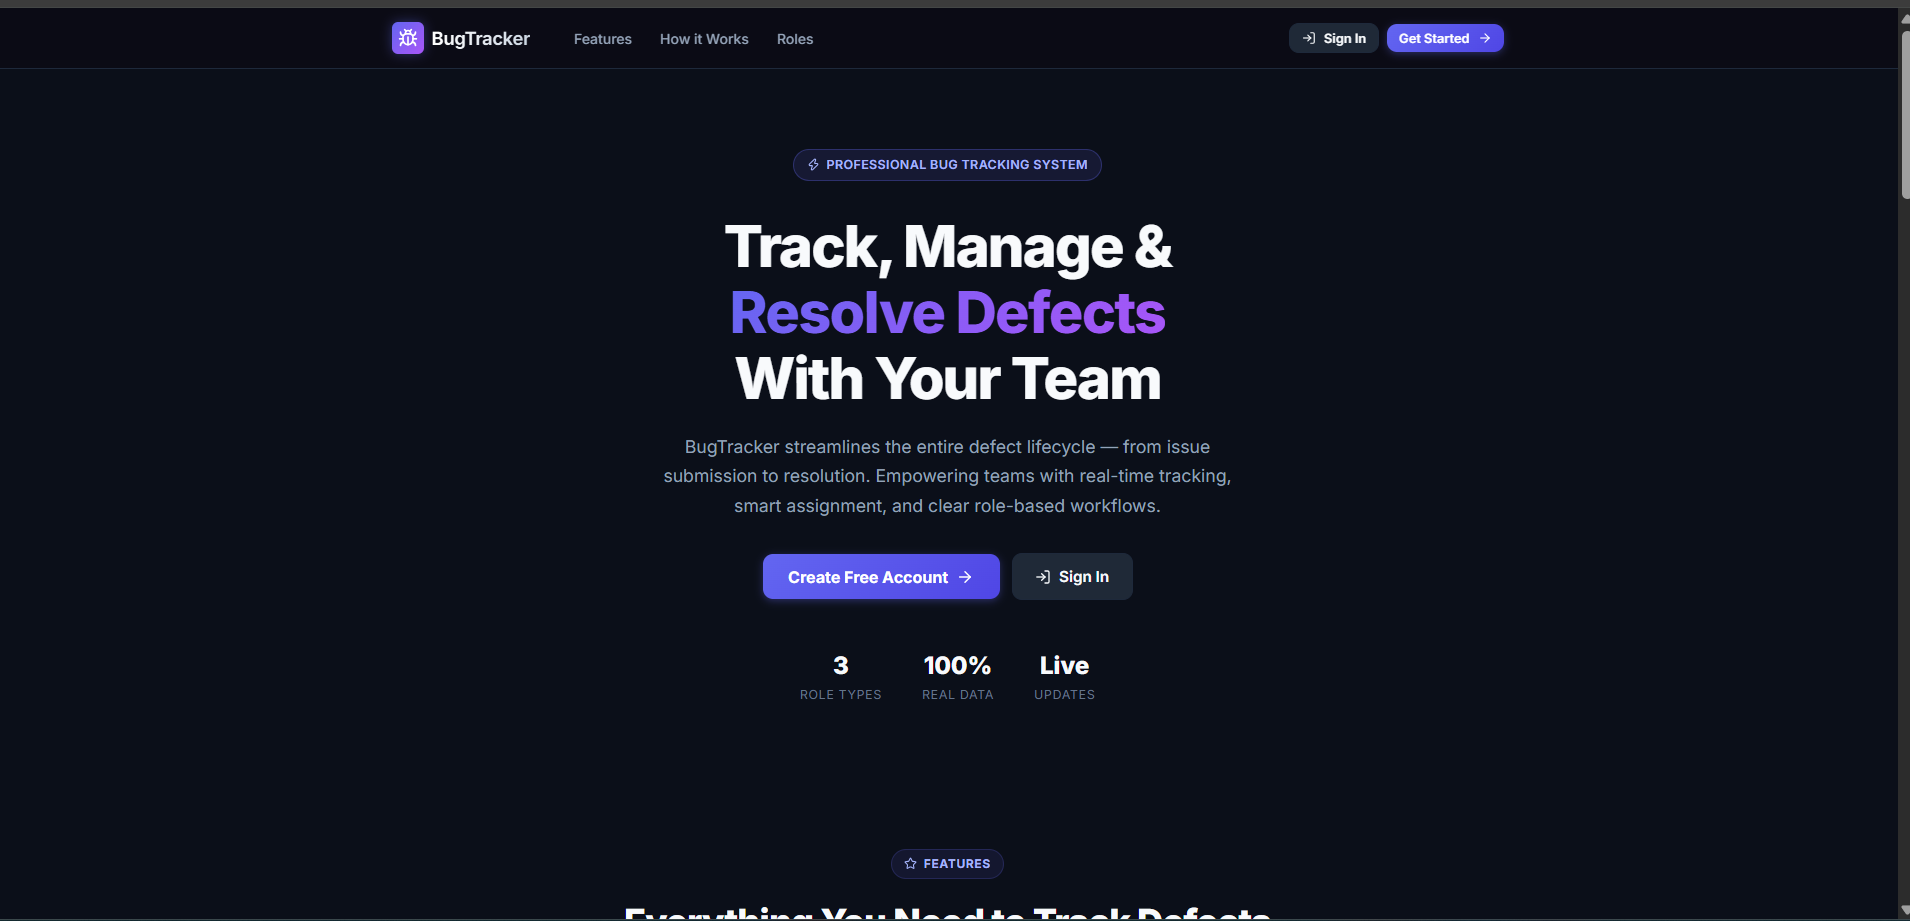
\includegraphics[width=\linewidth]{home.png}
    \caption{Landing Page}
    \label{fig:home}
  \end{minipage}%
  \hfill
  \begin{minipage}[t]{0.38\textwidth}
    \centering
    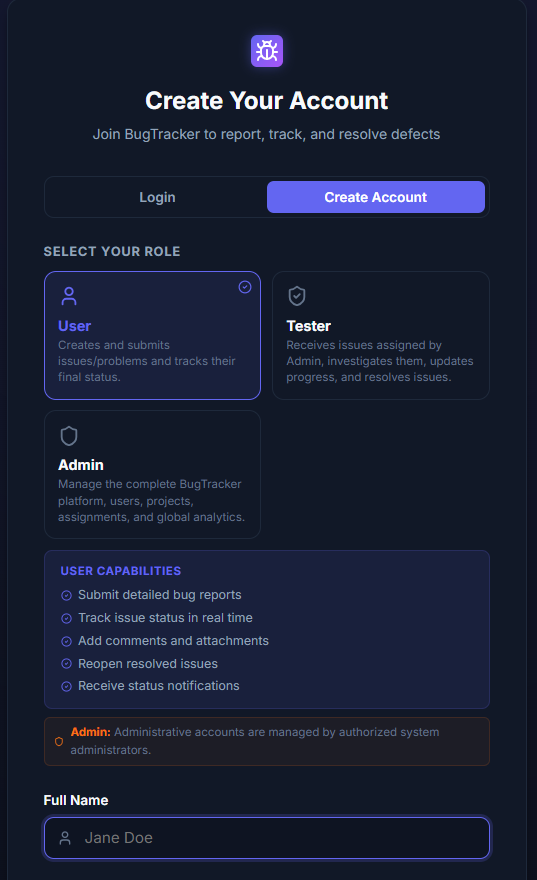
\includegraphics[width=\linewidth]{register.png}
    \caption{Registration Page}
    \label{fig:register}
  \end{minipage}
\end{figure}

% --- Page 2: All 3 Dashboards ---
\clearpage
\noindent\textbf{Role Dashboards}
\vspace{6pt}

\begin{figure}[htbp]
  \centering
  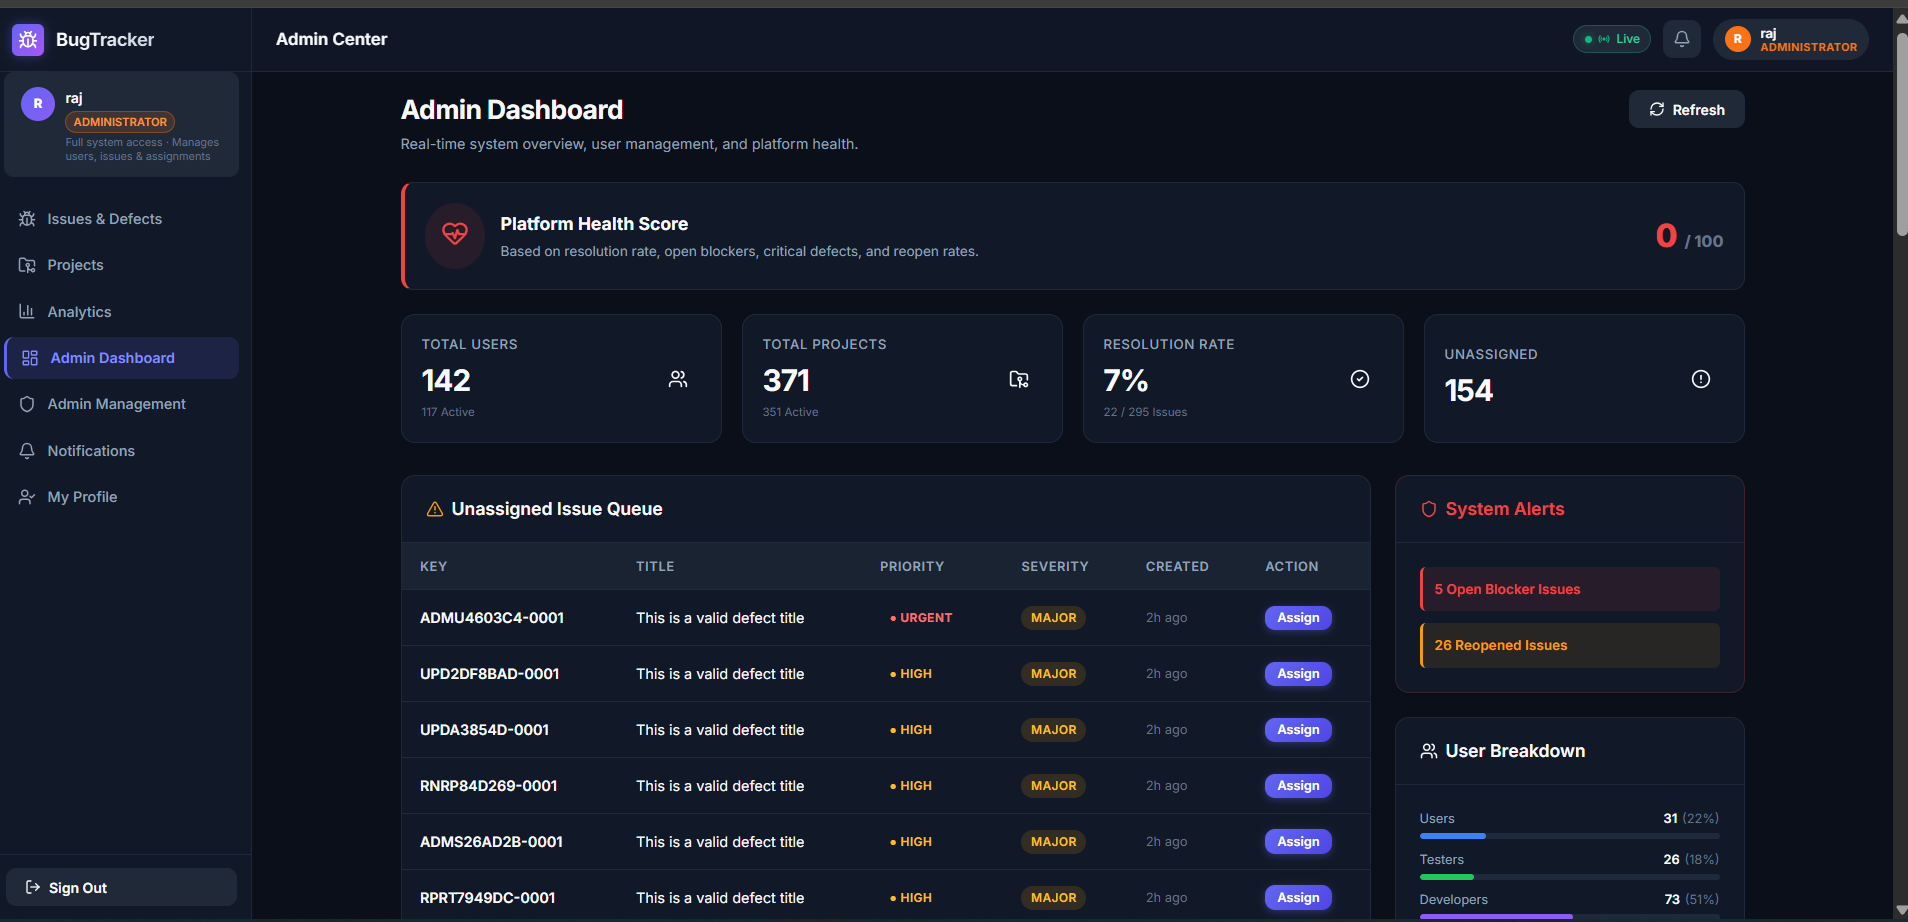
\includegraphics[width=0.92\textwidth]{admin_dash.png}
  \caption{Admin Dashboard --- Platform health score, unassigned issue queue, system alerts and user breakdown}
  \label{fig:admindash}
\end{figure}

\vspace{4pt}

\begin{figure}[htbp]
  \centering
  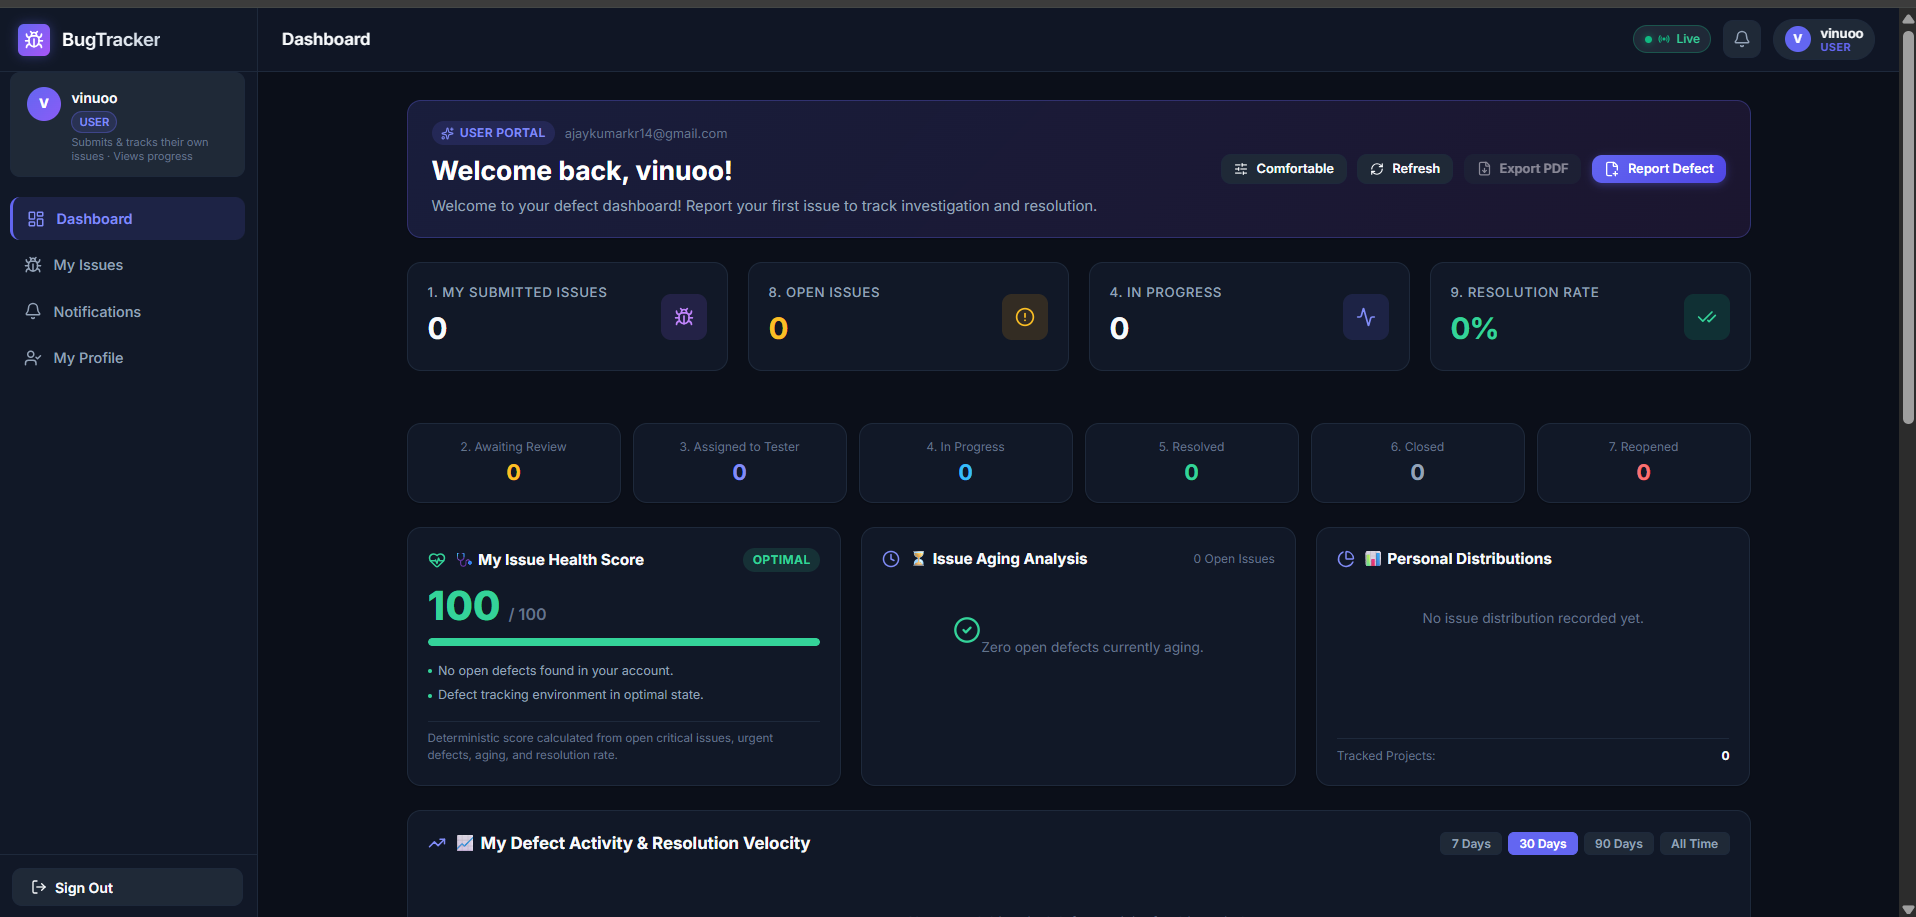
\includegraphics[width=0.92\textwidth]{user_dash.png}
  \caption{User Dashboard --- Issue health score, aging analysis and defect activity overview}
  \label{fig:userdash}
\end{figure}

\vspace{4pt}

\begin{figure}[htbp]
  \centering
  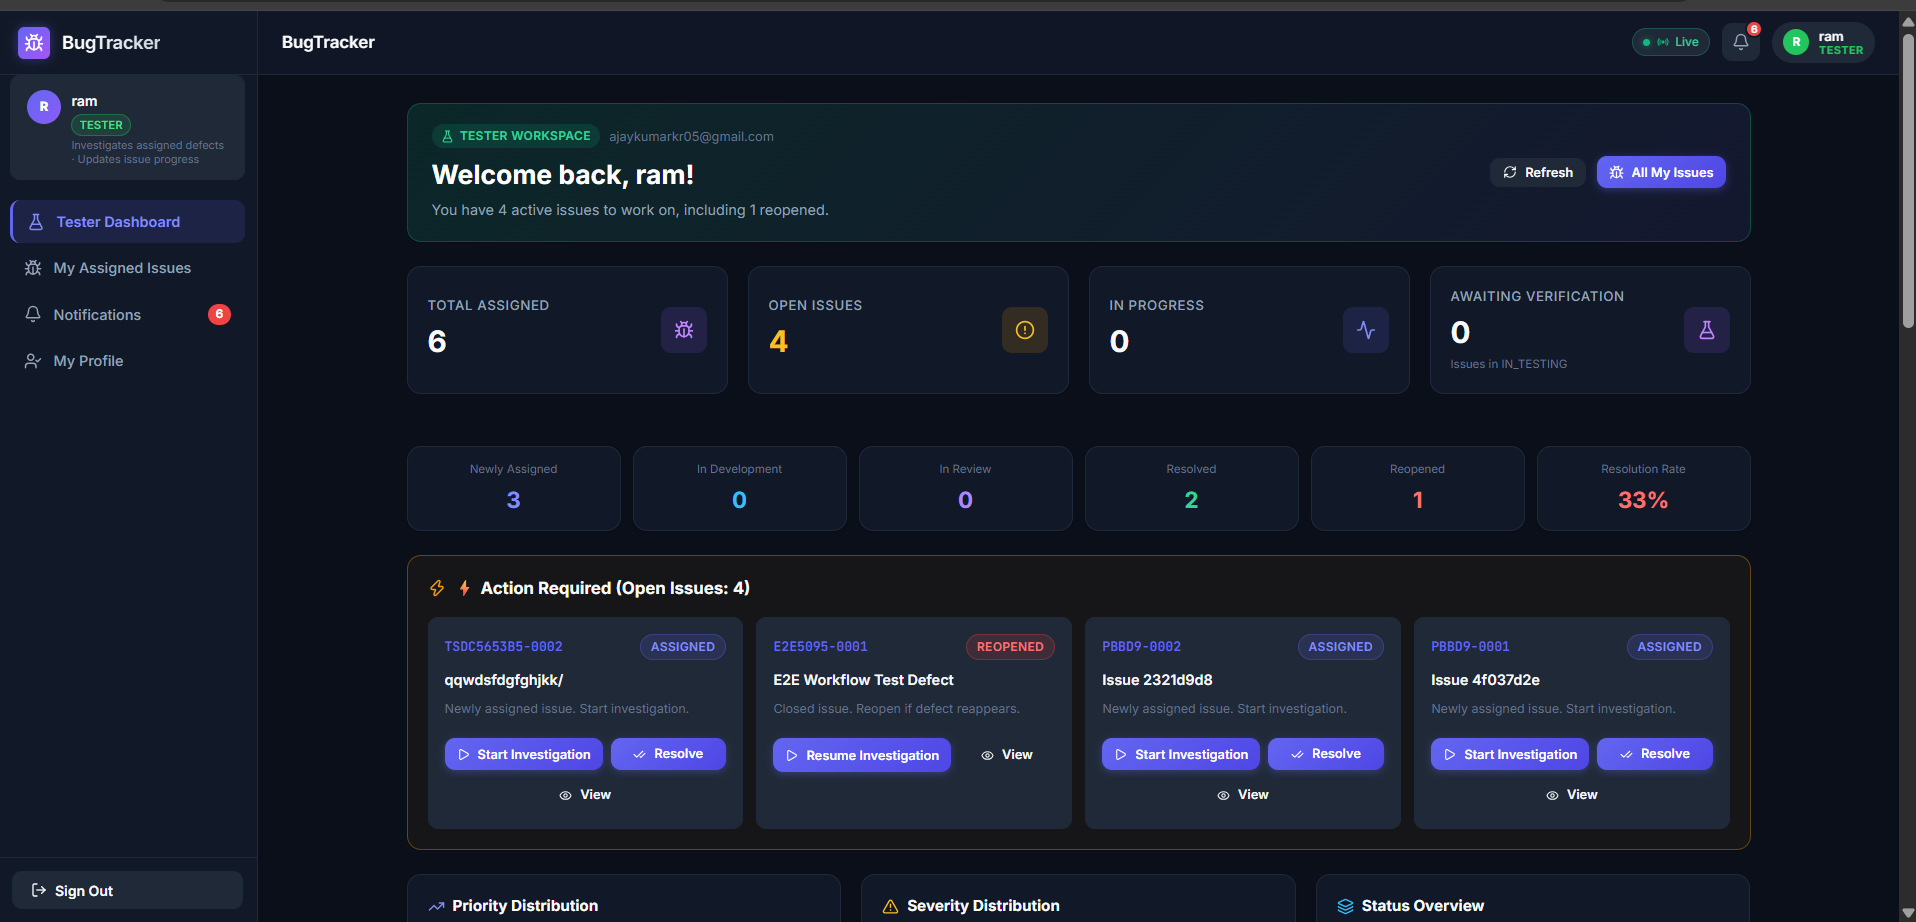
\includegraphics[width=0.92\textwidth]{testor.png}
  \caption{Tester Dashboard --- Action required queue with workflow buttons}
  \label{fig:testordash}
\end{figure}

% --- Page 3: Analytics ---
\clearpage
\begin{figure}[htbp]
  \centering
  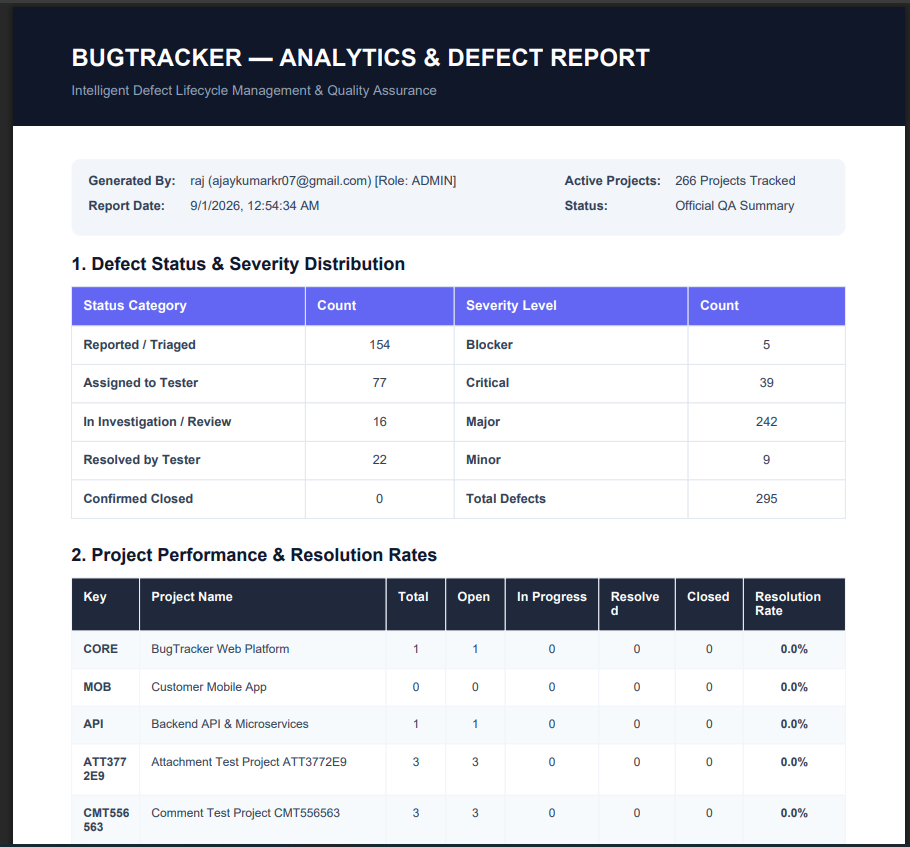
\includegraphics[width=\textwidth]{result.png}
  \caption{Analytics \& Defect Report --- Status distribution, severity breakdown and per-project resolution rates}
  \label{fig:analytics}
\end{figure}

\clearpage

% ===================== 9. DELIVERABLES =====================
\section{Deliverables \& Acceptance Criteria}

\renewcommand{\arraystretch}{1.25}
\rowcolors{2}{white}{rowalt}
\begin{tabular}{|L{11.8cm}|L{4cm}|}
\hline
\tblhead{Criterion} & \tblhead{Status} \\
\hline
PostgreSQL schema deployed across 7 core tables with indexes & Complete \\
\hline
JWT authentication with bcrypt password hashing & Complete \\
\hline
Role-based permissions across 3 roles enforced in UI and API & Complete \\
\hline
Duplicate detection on issue titles (Jaccard overlap, 0.4 threshold) & Complete \\
\hline
Rule-based auto-classification of issue type and severity & Complete \\
\hline
Real-time WebSocket notifications & Complete \\
\hline
Immutable, field-level audit log & Complete \\
\hline
Analytics APIs and CSV export & Complete \\
\hline
Auto-generated API documentation at /docs & Complete \\
\hline
Automated backend test suite (371 tests) & Complete \\
\hline
Email OTP verification enforcement at registration & Pending --- built, not yet enforced \\
\hline
\end{tabular}
\endrowcolors

% ===================== 10. LIMITATIONS & FUTURE WORK =====================
\section{Current Limitation \& Future Enhancements}

Email OTP Verification: the infrastructure for email OTP verification (database table, routes, OTP service, SMTP email sender) is fully built. In the current development build, however, accounts are activated immediately upon registration without requiring OTP confirmation. Email verification will be enforced in a future milestone.

\subsection{10.1 Future Enhancements}

\renewcommand{\arraystretch}{1.25}
\rowcolors{2}{white}{rowalt}
\begin{tabular}{|L{4.2cm}|L{11.6cm}|}
\hline
\tblhead{Feature} & \tblhead{Description} \\
\hline
Email OTP Activation & Enable the already-built OTP gate at registration \\
\hline
AI Defect Classification & Auto-suggest severity and priority from the issue description using an LLM \\
\hline
Server-Side Duplicate Detection & Backend NLP similarity search across all historical issues \\
\hline
Email Notifications & Send alerts via SMTP for offline users \\
\hline
Cloud Deployment & Deploy to a production environment with HTTPS \\
\hline
\end{tabular}
\endrowcolors

% ===================== 11. CONCLUSION =====================
\section{Conclusion}

In Module 1, the complete foundation of the Intelligent Software Defect Tracking System has been designed, built, and verified. The system supports the full User $\rightarrow$ Admin $\rightarrow$ Tester $\rightarrow$ User defect-management workflow with real-time WebSocket notifications, PostgreSQL persistence, role-based access control, comprehensive audit logging, and analytics. All 371 backend tests pass with zero failures, and the platform is fully functional in the local development environment, ready to support the enhancements planned for future milestones.

\vspace{1cm}
\begin{center}
\rule{0.9\textwidth}{0.4pt}\\[6pt]
{\small\itshape\color{gray666} Submitted by: Ajaykumar K R \ $|$\ Infosys Springboard Virtual Internship 7.0 \ $|$\ Batch 3}
\end{center}

\end{document}